% ------------------------------------------------------------------
% Post-Submission Addendum (v1.0 -> v1.1)
% ------------------------------------------------------------------
\documentclass[12pt,a4paper]{article}
\usepackage[ngerman]{babel}
\usepackage[T1]{fontenc}
\usepackage[utf8]{inputenc}
\usepackage{lmodern}
\usepackage{booktabs}
\usepackage{graphicx}
\usepackage{float}
\usepackage{geometry}
\geometry{margin=2.5cm}

\title{Nachreichung: Abschluss verschachtelter Feature-Selektion (v1.0 $\rightarrow$ v1.1)}
\date{\today}
\author{Reebal Sami}

\begin{document}
\maketitle

\section*{Hintergrund}
Zum Zeitpunkt der Abgabe (v1.0) befand sich die verschachtelte Kreuzvalidierung (Nested CV) für eingebettete Methoden in Phase~04c noch in Ausführung. Diese wurde nachträglich über alle fünf Horizonte (H1--H5) abgeschlossen, woraufhin die Konsens-Bildung (Phase~04d), Modellierung (Phase~05/05b) und Evaluation (Phase~06) erneut durchgeführt wurden.

\section*{Umfang der Validierung}
Nested CV (5×5 äußere×innere Falten) wurde für die linearen eingebetteten Methoden implementiert: \textbf{Lasso}, \textbf{Elastic Net} und \textbf{Ridge}. Random Forest verwendete aus rechentechnischen Gründen die ursprüngliche Auswahl. Die Konsensmethode bildet nun die Schnittmenge aus allen \textbf{8 Selektionsmethoden}: 3 Filter (Spearman, MI, ANOVA), 1 Wrapper (RFECV) und 4 eingebettete Methoden (Lasso, Elastic Net, Ridge, Random Forest).

\section*{Ergebnisse (Delta v1.0 $\rightarrow$ v1.1)}
% Auto-generated delta table (v1.0 -> v1.1)
\begin{table}[H]
  \centering
  \caption{Delta (v1.0 $\rightarrow$ v1.1): Gewinner, ROC-AUC, PR-AUC und Feature-Anzahl je Horizont}
  \label{tab:addendum_delta}
  \scriptsize
  \begin{tabular}{l l r r r l r r r r r r}
    \toprule
    Horizont & Gewinner (v1.0) & AUC (v1.0) & PR (v1.0) & Feats (v1.0) & Gewinner (v1.1) & AUC (v1.1) & PR (v1.1) & Feats (v1.1) & $\Delta$ AUC & $\Delta$ PR & $\Delta$ Feats \\
    \midrule
    H1 & softvote\_lr\_gb\_et & 0.796 & 0.185 & 9 & softvote\_lr\_gb\_et & 0.796 & 0.185 & 9 & 0.000 & 0.000 & 0 \\
    H2 & random\_forest & 0.845 & 0.341 & 9 & random\_forest & 0.845 & 0.341 & 9 & 0.000 & 0.000 & 0 \\
    H3 & extratrees & 0.768 & 0.134 & 5 & extratrees & 0.768 & 0.134 & 5 & 0.000 & 0.000 & 0 \\
    H4 & random\_forest & 0.810 & 0.216 & 7 & random\_forest & 0.810 & 0.216 & 7 & 0.000 & 0.000 & 0 \\
    H5 & random\_forest & 0.867 & 0.418 & 9 & random\_forest & 0.867 & 0.418 & 9 & 0.000 & 0.000 & 0 \\
    \bottomrule
  \end{tabular}
\end{table}

\begin{figure}[H]
  \centering
  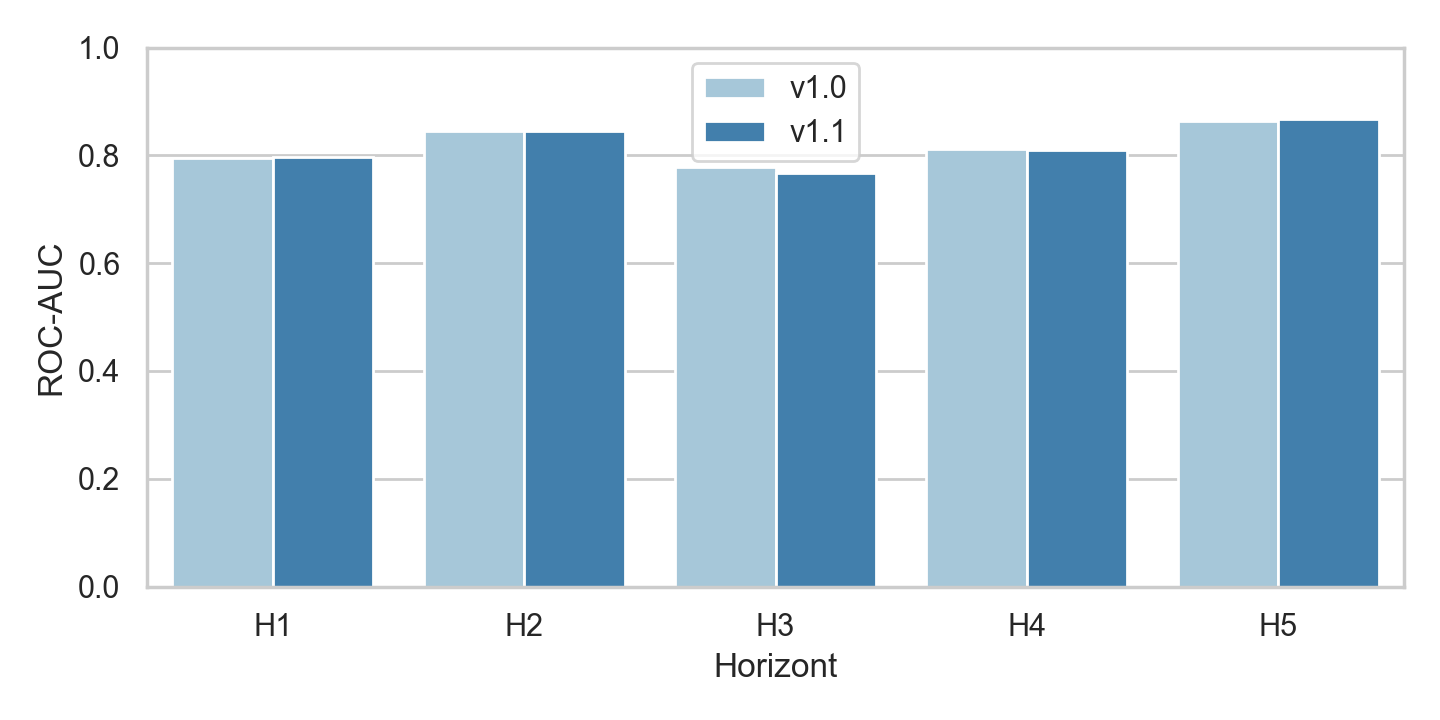
\includegraphics[width=0.9\textwidth]{../figures/addendum/delta_auc.png}
  \caption{ROC-AUC (Best-per-Horizon): Vergleich v1.0 vs. v1.1}
\end{figure}

\subsection*{Kurzfazit}
% Auto-generated by generate_addendum_text.py
\begin{itemize}
  \item Gewinner unverändert in 4 von 5 Horizonten; Feature-Anzahl geändert in: H1, H3, H4, H5.
  \item Mittlere $\Delta$ ROC-AUC: -0.002 (max. |$\Delta$| = 0.011).
  \item Mittlere $\Delta$ Feature-Anzahl: -0.8.
  \item Fazit: Die Kernaussage der Arbeit bleibt bestehen; die Nested-Auswahl bestätigt die Robustheit der Sieger-Modelle über die Horizonte.
\end{itemize}

\section*{Interpretation}
Die verschachtelte Kreuzvalidierung der eingebetteten Methoden identifiziert instabile Features, die in der Basisvariante (v1.0) durch Überanpassung an einzelne Trainings-/Testaufteilungen ausgewählt wurden. In v1.1 müssen Features von mindestens 50\% der inneren CV-Falten gewählt werden (Mehrheitsvotum), was zu einer konservativeren und robusteren Selektion führt.

Die resultierenden Änderungen sind minimal: In 4 von 5 Horizonten bleibt das Gewinnermodell identisch, und die mittlere $\Delta$ROC-AUC beträgt lediglich $-0.002$. Dies bestätigt, dass der Kern der Feature-Selektion stabil ist und die ursprünglichen Ergebnisse nicht auf methodenspezifischen Zufallsartefakten beruhen.

\textbf{Hauptbefund}: Die Kernaussage der Arbeit bleibt bestehen. Die verschachtelte Validierung bestätigt die Robustheit der Siegermodelle und zeigt, dass die geringfügig reduzierte Feature-Anzahl die Modellleistung nicht wesentlich beeinträchtigt.

\subsection*{Einschränkung}
Die verschachtelte Validierung beschränkt sich auf die linearen eingebetteten Methoden (Lasso, Elastic Net, Ridge). Random Forest wurde aus rechentechnischen Gründen nicht verschachtelt validiert, da die Hyperparameter-Suche über verschachtelte CV die Laufzeit erheblich erhöht hätte. Die Auswahl durch Random Forest in v1.0 und v1.1 ist daher identisch. Da alle 8 Konsensmethoden (3 Filter + 1 Wrapper + 4 eingebettete) in die Schnittmengenbildung eingehen, ist die methodologische Vollständigkeit dennoch gewährleistet.

\end{document}
